\section{System Design}
\label{sec:design}
The runtime exposes named operations through two paths (Fig.~\ref{fig:arch}). In a task, a registered agent harness is the adapter that exposes scoped tools for data acquisition (DAQ) and intent submission. An agent uses observations and the task objective to analyze what to propose; it does not decide whether a write is authorized. Direct representational state transfer (REST) or stdio MCP calls invoke operations without a task. The architecture routes both entries through one dispatcher; Section~\ref{sec:eval} tests selected direct calls, not equivalent behavior across both entries.

\begin{figure*}[!t]
\centering
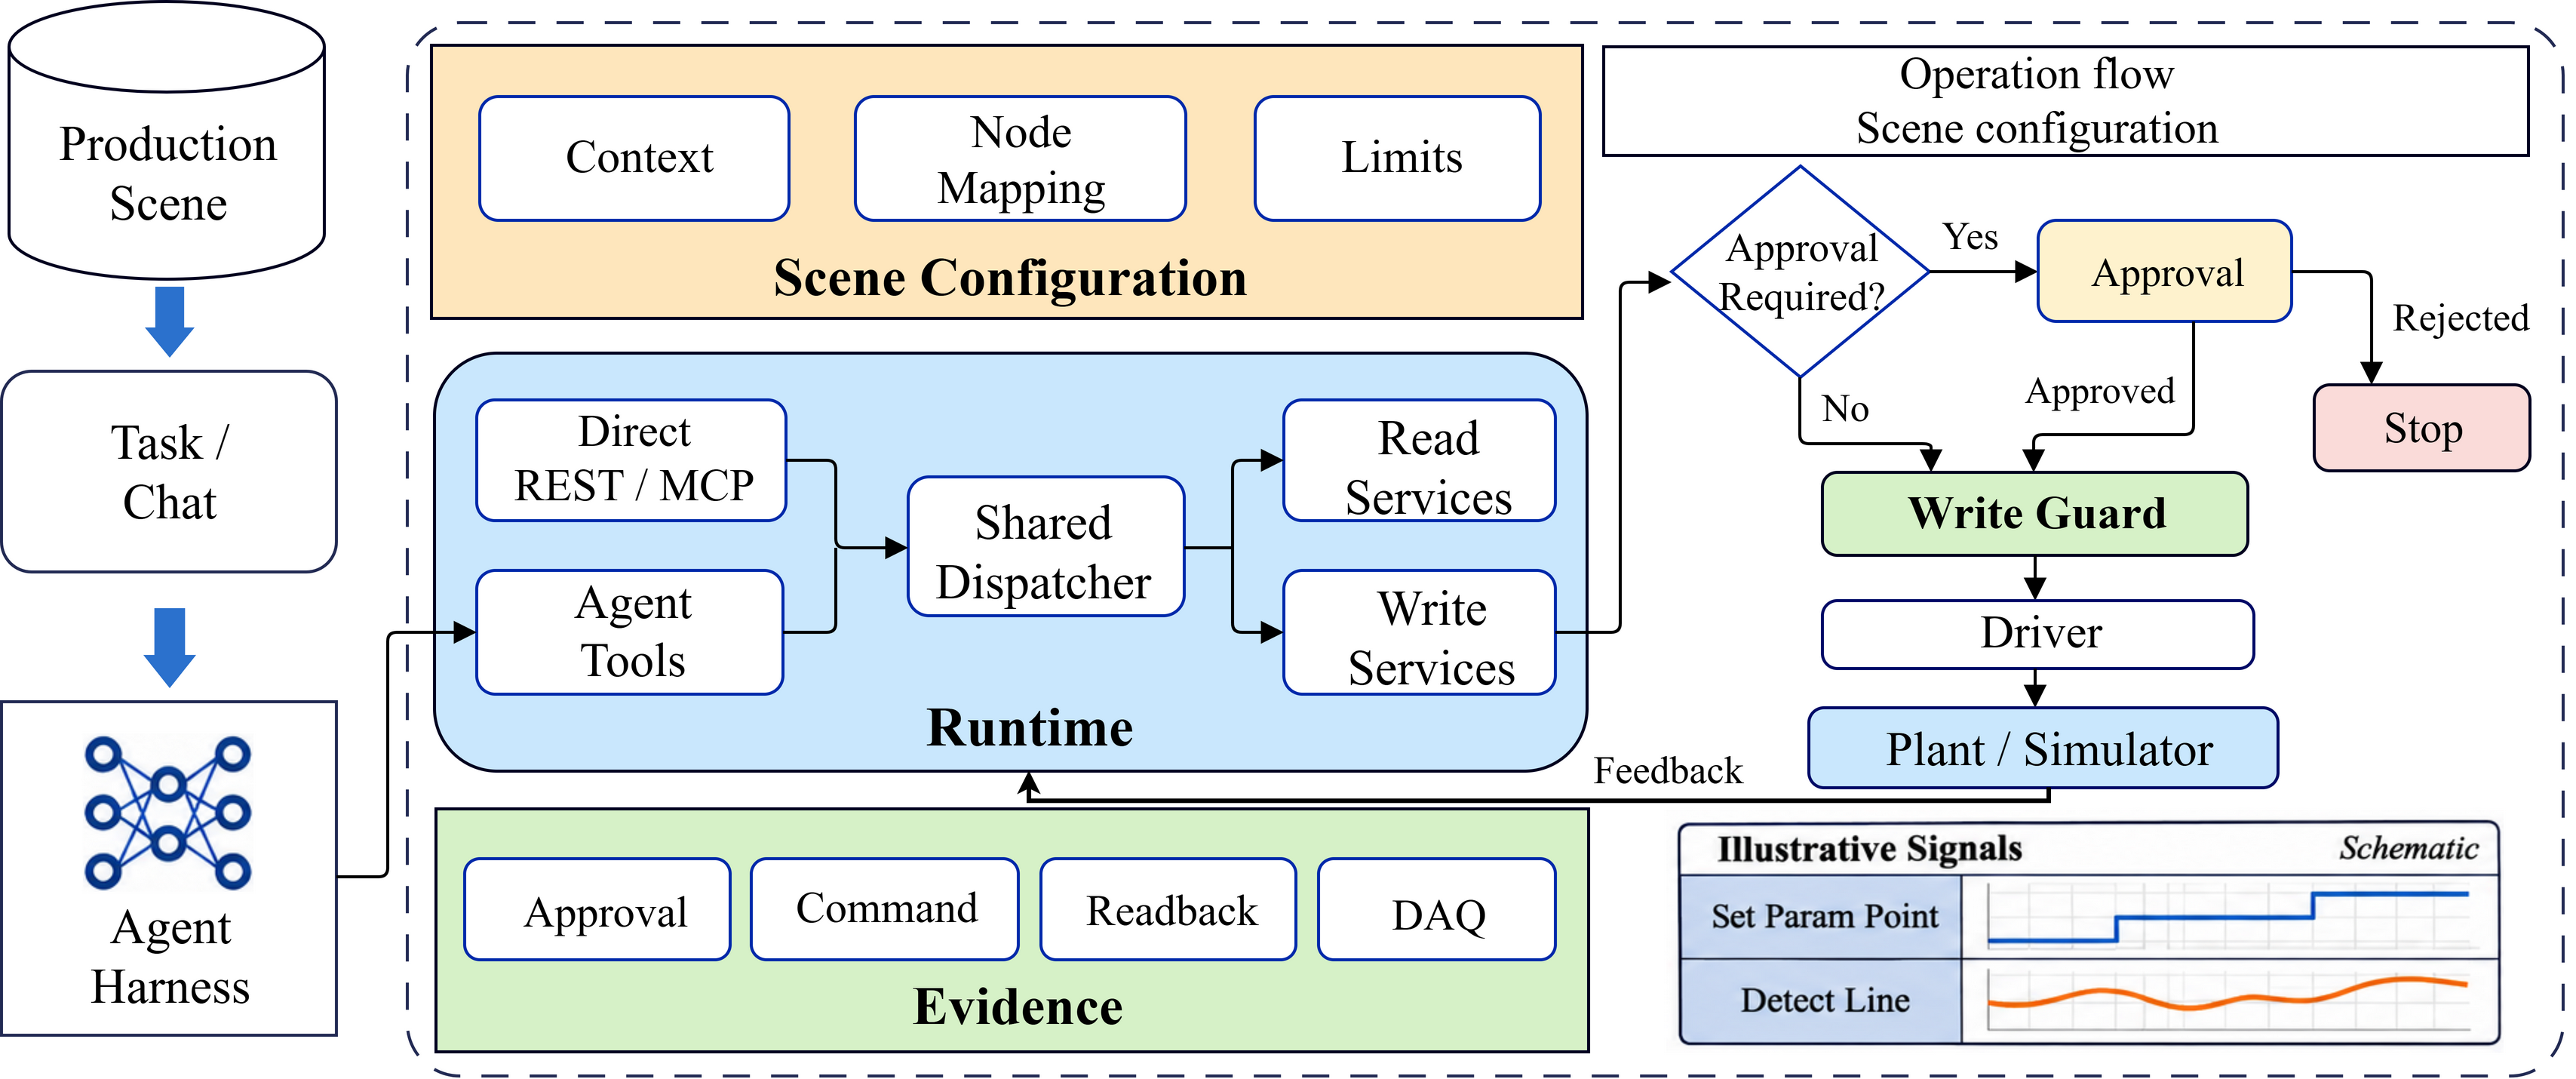
\includegraphics[width=\textwidth]{resources/fig2.png}
\caption{Task-mediated and direct tool calls share a dispatcher; a registered agent can acquire observations and submit a control intent, while direct calls provide a test entry point. Direct calls do not require a task. Approved intents undergo route-specific revalidation (omitted here; see Fig.~\ref{fig:hitl}). The no-approval path remains subject to applicable authorization and write guards. Requests rejected by pre-dispatch checks stop before driver dispatch. Feedback and signals are schematic, not measured traces. Approvals, command outcomes, optional readbacks, and later data-acquisition (DAQ) observations are distinct records. In-flight exclusion of overlapping writes per node and process is not shown; equipment interlocks remain necessary.}
\label{fig:arch}
\end{figure*}

\subsection{Design Rationale and Requirements}
\label{sec:principles}
The runtime must preserve process meaning across heterogeneous drivers, hold a stable contract for registered harness adapters, and check authority and process limits before every control write, keeping acquired process data, command acceptance, and later observations distinct. Scene configuration, registered adapters, shared dispatch, route handlers, and service-owned records enforce these boundaries.

For each agent turn, the context builder assembles the production context and eligible observations. The agent uses them to shape a proposal, but neither context nor observations grant write authority; the handler resolves live state when the operation is invoked.

\subsection{Layered Architecture}
\label{sec:layers}
Fig.~\ref{fig:arch} shows the layers: task and chat routes use registered harness adapters providing scoped acquisition and control tools, constrained by binding and by the policy of the agent's channel, its scoped execution context; agent analysis remains distinct from deterministic boundary checks, and the feedback path and signals are schematic.

Direct REST agent-tool calls and the stdio-MCP bridge bypass task execution and enter the shared dispatcher. The task route gives the agent context, acquisition targets, and objectives; operation services resolve control mappings and guards. Read and analysis services---DAQ, MES access, retrieval, and optional model services---are separated from write and recipe services. Input/output mappings connect semantic nodes to built-in or plugin drivers, and owning services retain task, command, observation, and configuration records.

\subsection{Scene Configuration as the Integration Boundary}
\label{sec:scene-config}
Scene-specific semantics are configured before use: the active line identifies the production context, product and recipe records supply applicable targets and limits, and the run record provides the current operating state. Semantic nodes bind process variables to direction-specific acquisition or control mappings, which the driver registry resolves to protocol implementations; \emph{semantic} here denotes a named process variable with a direction, unit, and configured mapping, not an OPC UA or Asset Administration Shell information model. Each agent-facing operation is named and typed, so a harness need not construct protocol-specific messages; a scene using a registered driver can supply different context and node mappings behind the same operation contract, while a protocol absent from the registry still requires a driver adapter.

In the cast-film preset, the MQTT command mapping \texttt{linespeed-sp} controls line speed in m/min, while the distinct \texttt{film-thickness} mapping reads thickness in $\mu$m; an agent can acquire the thickness observation, compare it with its objective, and propose a line-speed intent, which the runtime admits against the control node's limits. Sharing MQTT does not make either signal a substitute for the other.

Table~\ref{tab:scene-config} summarizes how the execution path uses the scene description, distinguishing configuration-time bindings from live-state checks. The context for an agent turn describes the active scene; before a write, the handler resolves the route's live state, applies current limits, and binds approval to both proposal and context where snapshots are supported (Section~\ref{sec:modules}). The command receipt remains separate from subsequent DAQ observations.

\begin{table*}[!t]
\centering
\caption{Scene configuration elements and their roles in the runtime path.}
\label{tab:scene-config}
\footnotesize
\setlength{\tabcolsep}{5pt}
\begin{tabularx}{\textwidth}{@{}>{\raggedright\arraybackslash}p{0.19\textwidth}>{\raggedright\arraybackslash}p{0.34\textwidth}X@{}}
\toprule
Element & Configured information & Runtime use\\
\midrule
Production context & Line, product, recipe, and run associations & Context construction for a task turn; route-dependent live-state checks before a write\\
Semantic I/O & Process variable, direction, unit, and node mapping & Acquisition uses the read mapping; accepted operations resolve the configured control mapping\\
Driver binding & Supported protocol driver and endpoint configuration & Driver registry selects the protocol implementation after operation checks\\
Operation admission & Engineering, baseline, product, and recipe limits; step and timing rules where configured & Route handler checks the candidate against current bounds and rejects inadmissible requests\\
Approval policy & Whether approval is required and the decision validity window & Pending request binds the proposed action; route-specific checks run after approval\\
Evidence ownership & Command receipt, verification grade, and later DAQ observations & Owning services retain command outcomes separately from process measurements\\
\bottomrule
\end{tabularx}
\end{table*}

\subsection{Cross-Module Execution Flow}
\label{sec:executionflow}
For a task-mediated call, the registered adapter presents a scoped tool
catalog containing acquisition, context, and control operations to the agent.
The agent reads available observations, relates them to the task objective, and
submits a typed intent rather than a protocol-specific message. At the
operation boundary, the shared dispatcher checks the predicates declared for
the named operation before selecting its handler. The handler resolves live
production state, applies route-specific guards and limits, and requests any
required approval before device I/O.

For an industrial operation $u$ by agent $a$ in channel $c$, the shared dispatch condition is
\begin{equation}
\mathcal{A}(a,c,u)=\bigwedge_{X\in\mathcal{C}(u)}X(a,c,u).
\label{eq:dispatch-contract}
\end{equation}
The dispatch predicates $S$, $P$, $G$, and $B$ in Eq.~(\ref{eq:dispatch-contract}) denote invocation scope, current channel policy,
the applicable industrial grant, and the agent's binding to referenced resources,
respectively. The declared set $\mathcal{C}(u)\subseteq\{S,P,G,B\}$ always contains
$S$ and $P$; the grant predicate $G$ joins when the resolved channel, target line, and owner/grant policy
require it, and the binding predicate $B$ joins when the operation declares resource references. Every included check must pass before handler
selection. Where configured, the policy predicate also covers channel tool
selection, profile, and duty-separation checks.

Once these predicates pass, the selected route applies its operational
guards and requests any required approval. For example, an exploration request checks
the control binding and DAQ visibility before entering the governed write
path; an invisible target returns an error before a write. The checks performed
after approval depend on the route; Section~\ref{sec:modules} specifies the
single-node and recipe-operation paths.

For a direct REST agent-tool call, the service establishes $a$ and $c$ before applying these checks: an agent token must match the requested agent identifier, an authenticated user must be the channel owner or an administrator, and the manager then loads the channel-agent record, rechecking scope and policy with any applicable grant and binding checks. Handlers resolve live production state
from request identifiers and the owning services.


